
%% bare_jrnl_compsoc.tex
%% V1.4b
%% 2015/08/26
%% by Michael Shell
%% See:
%% http://www.michaelshell.org/
%% for current contact information.
%%
%% This is a skeleton file demonstrating the use of IEEEtran.cls
%% (requires IEEEtran.cls version 1.8b or later) with an IEEE
%% Computer Society journal paper.
%%
%% Support sites:
%% http://www.michaelshell.org/tex/ieeetran/
%% http://www.ctan.org/pkg/ieeetran
%% and
%% http://www.ieee.org/

%%*************************************************************************
%% Legal Notice:
%% This code is offered as-is without any warranty either expressed or
%% implied; without even the implied warranty of MERCHANTABILITY or
%% FITNESS FOR A PARTICULAR PURPOSE! 
%% User assumes all risk.
%% In no event shall the IEEE or any contributor to this code be liable for
%% any damages or losses, including, but not limited to, incidental,
%% consequential, or any other damages, resulting from the use or misuse
%% of any information contained here.
%%
%% All comments are the opinions of their respective authors and are not
%% necessarily endorsed by the IEEE.
%%
%% This work is distributed under the LaTeX Project Public License (LPPL)
%% ( http://www.latex-project.org/ ) version 1.3, and may be freely used,
%% distributed and modified. A copy of the LPPL, version 1.3, is included
%% in the base LaTeX documentation of all distributions of LaTeX released
%% 2003/12/01 or later.
%% Retain all contribution notices and credits.
%% ** Modified files should be clearly indicated as such, including  **
%% ** renaming them and changing author support contact information. **
%%*************************************************************************


% *** Authors should verify (and, if needed, correct) their LaTeX system  ***
% *** with the testflow diagnostic prior to trusting their LaTeX platform ***
% *** with production work. The IEEE's font choices and paper sizes can   ***
% *** trigger bugs that do not appear when using other class files.       ***                          ***
% The testflow support page is at:
% http://www.michaelshell.org/tex/testflow/


\documentclass[10pt,journal,compsoc]{IEEEtran}
%
% If IEEEtran.cls has not been installed into the LaTeX system files,
% manually specify the path to it like:
% \documentclass[10pt,journal,compsoc]{../sty/IEEEtran}





% Some very useful LaTeX packages include:
% (uncomment the ones you want to load)


% *** MISC UTILITY PACKAGES ***
%
%\usepackage{ifpdf}
% Heiko Oberdiek's ifpdf.sty is very useful if you need conditional
% compilation based on whether the output is pdf or dvi.
% usage:
% \ifpdf
%   % pdf code
% \else
%   % dvi code
% \fi
% The latest version of ifpdf.sty can be obtained from:
% http://www.ctan.org/pkg/ifpdf
% Also, note that IEEEtran.cls V1.7 and later provides a builtin
% \ifCLASSINFOpdf conditional that works the same way.
% When switching from latex to pdflatex and vice-versa, the compiler may
% have to be run twice to clear warning/error messages.






% *** CITATION PACKAGES ***
%
\ifCLASSOPTIONcompsoc
  % IEEE Computer Society needs nocompress option
  % requires cite.sty v4.0 or later (November 2003)
  \usepackage[nocompress]{cite}
\else
  % normal IEEE
  \usepackage{cite}
\fi
% cite.sty was written by Donald Arseneau
% V1.6 and later of IEEEtran pre-defines the format of the cite.sty package
% \cite{} output to follow that of the IEEE. Loading the cite package will
% result in citation numbers being automatically sorted and properly
% "compressed/ranged". e.g., [1], [9], [2], [7], [5], [6] without using
% cite.sty will become [1], [2], [5]--[7], [9] using cite.sty. cite.sty's
% \cite will automatically add leading space, if needed. Use cite.sty's
% noadjust option (cite.sty V3.8 and later) if you want to turn this off
% such as if a citation ever needs to be enclosed in parenthesis.
% cite.sty is already installed on most LaTeX systems. Be sure and use
% version 5.0 (2009-03-20) and later if using hyperref.sty.
% The latest version can be obtained at:
% http://www.ctan.org/pkg/cite
% The documentation is contained in the cite.sty file itself.
%
% Note that some packages require special options to format as the Computer
% Society requires. In particular, Computer Society  papers do not use
% compressed citation ranges as is done in typical IEEE papers
% (e.g., [1]-[4]). Instead, they list every citation separately in order
% (e.g., [1], [2], [3], [4]). To get the latter we need to load the cite
% package with the nocompress option which is supported by cite.sty v4.0
% and later. Note also the use of a CLASSOPTION conditional provided by
% IEEEtran.cls V1.7 and later.





% *** GRAPHICS RELATED PACKAGES ***
%
\ifCLASSINFOpdf
  % \usepackage[pdftex]{graphicx}
  % declare the path(s) where your graphic files are
  % \graphicspath{{../pdf/}{../jpeg/}}
  % and their extensions so you won't have to specify these with
  % every instance of \includegraphics
  % \DeclareGraphicsExtensions{.pdf,.jpeg,.png}
\else
  % or other class option (dvipsone, dvipdf, if not using dvips). graphicx
  % will default to the driver specified in the system graphics.cfg if no
  % driver is specified.
  % \usepackage[dvips]{graphicx}
  % declare the path(s) where your graphic files are
  % \graphicspath{{../eps/}}
  % and their extensions so you won't have to specify these with
  % every instance of \includegraphics
  % \DeclareGraphicsExtensions{.eps}
\fi
% graphicx was written by David Carlisle and Sebastian Rahtz. It is
% required if you want graphics, photos, etc. graphicx.sty is already
% installed on most LaTeX systems. The latest version and documentation
% can be obtained at: 
% http://www.ctan.org/pkg/graphicx
% Another good source of documentation is "Using Imported Graphics in
% LaTeX2e" by Keith Reckdahl which can be found at:
% http://www.ctan.org/pkg/epslatex
%
% latex, and pdflatex in dvi mode, support graphics in encapsulated
% postscript (.eps) format. pdflatex in pdf mode supports graphics
% in .pdf, .jpeg, .png and .mps (metapost) formats. Users should ensure
% that all non-photo figures use a vector format (.eps, .pdf, .mps) and
% not a bitmapped formats (.jpeg, .png). The IEEE frowns on bitmapped formats
% which can result in "jaggedy"/blurry rendering of lines and letters as
% well as large increases in file sizes.
%
% You can find documentation about the pdfTeX application at:
% http://www.tug.org/applications/pdftex






% *** MATH PACKAGES ***
%
%\usepackage{amsmath}
% A popular package from the American Mathematical Society that provides
% many useful and powerful commands for dealing with mathematics.
%
% Note that the amsmath package sets \interdisplaylinepenalty to 10000
% thus preventing page breaks from occurring within multiline equations. Use:
%\interdisplaylinepenalty=2500
% after loading amsmath to restore such page breaks as IEEEtran.cls normally
% does. amsmath.sty is already installed on most LaTeX systems. The latest
% version and documentation can be obtained at:
% http://www.ctan.org/pkg/amsmath





% *** SPECIALIZED LIST PACKAGES ***
%
%\usepackage{algorithmic}
% algorithmic.sty was written by Peter Williams and Rogerio Brito.
% This package provides an algorithmic environment fo describing algorithms.
% You can use the algorithmic environment in-text or within a figure
% environment to provide for a floating algorithm. Do NOT use the algorithm
% floating environment provided by algorithm.sty (by the same authors) or
% algorithm2e.sty (by Christophe Fiorio) as the IEEE does not use dedicated
% algorithm float types and packages that provide these will not provide
% correct IEEE style captions. The latest version and documentation of
% algorithmic.sty can be obtained at:
% http://www.ctan.org/pkg/algorithms
% Also of interest may be the (relatively newer and more customizable)
% algorithmicx.sty package by Szasz Janos:
% http://www.ctan.org/pkg/algorithmicx




% *** ALIGNMENT PACKAGES ***
%
%\usepackage{array}
% Frank Mittelbach's and David Carlisle's array.sty patches and improves
% the standard LaTeX2e array and tabular environments to provide better
% appearance and additional user controls. As the default LaTeX2e table
% generation code is lacking to the point of almost being broken with
% respect to the quality of the end results, all users are strongly
% advised to use an enhanced (at the very least that provided by array.sty)
% set of table tools. array.sty is already installed on most systems. The
% latest version and documentation can be obtained at:
% http://www.ctan.org/pkg/array


% IEEEtran contains the IEEEeqnarray family of commands that can be used to
% generate multiline equations as well as matrices, tables, etc., of high
% quality.




% *** SUBFIGURE PACKAGES ***
%\ifCLASSOPTIONcompsoc
%  \usepackage[caption=false,font=footnotesize,labelfont=sf,textfont=sf]{subfig}
%\else
%  \usepackage[caption=false,font=footnotesize]{subfig}
%\fi
% subfig.sty, written by Steven Douglas Cochran, is the modern replacement
% for subfigure.sty, the latter of which is no longer maintained and is
% incompatible with some LaTeX packages including fixltx2e. However,
% subfig.sty requires and automatically loads Axel Sommerfeldt's caption.sty
% which will override IEEEtran.cls' handling of captions and this will result
% in non-IEEE style figure/table captions. To prevent this problem, be sure
% and invoke subfig.sty's "caption=false" package option (available since
% subfig.sty version 1.3, 2005/06/28) as this is will preserve IEEEtran.cls
% handling of captions.
% Note that the Computer Society format requires a sans serif font rather
% than the serif font used in traditional IEEE formatting and thus the need
% to invoke different subfig.sty package options depending on whether
% compsoc mode has been enabled.
%
% The latest version and documentation of subfig.sty can be obtained at:
% http://www.ctan.org/pkg/subfig




% *** FLOAT PACKAGES ***
%
%\usepackage{fixltx2e}
% fixltx2e, the successor to the earlier fix2col.sty, was written by
% Frank Mittelbach and David Carlisle. This package corrects a few problems
% in the LaTeX2e kernel, the most notable of which is that in current
% LaTeX2e releases, the ordering of single and double column floats is not
% guaranteed to be preserved. Thus, an unpatched LaTeX2e can allow a
% single column figure to be placed prior to an earlier double column
% figure.
% Be aware that LaTeX2e kernels dated 2015 and later have fixltx2e.sty's
% corrections already built into the system in which case a warning will
% be issued if an attempt is made to load fixltx2e.sty as it is no longer
% needed.
% The latest version and documentation can be found at:
% http://www.ctan.org/pkg/fixltx2e


%\usepackage{stfloats}
% stfloats.sty was written by Sigitas Tolusis. This package gives LaTeX2e
% the ability to do double column floats at the bottom of the page as well
% as the top. (e.g., "\begin{figure*}[!b]" is not normally possible in
% LaTeX2e). It also provides a command:
%\fnbelowfloat
% to enable the placement of footnotes below bottom floats (the standard
% LaTeX2e kernel puts them above bottom floats). This is an invasive package
% which rewrites many portions of the LaTeX2e float routines. It may not work
% with other packages that modify the LaTeX2e float routines. The latest
% version and documentation can be obtained at:
% http://www.ctan.org/pkg/stfloats
% Do not use the stfloats baselinefloat ability as the IEEE does not allow
% \baselineskip to stretch. Authors submitting work to the IEEE should note
% that the IEEE rarely uses double column equations and that authors should try
% to avoid such use. Do not be tempted to use the cuted.sty or midfloat.sty
% packages (also by Sigitas Tolusis) as the IEEE does not format its papers in
% such ways.
% Do not attempt to use stfloats with fixltx2e as they are incompatible.
% Instead, use Morten Hogholm'a dblfloatfix which combines the features
% of both fixltx2e and stfloats:
%
% \usepackage{dblfloatfix}
% The latest version can be found at:
% http://www.ctan.org/pkg/dblfloatfix




%\ifCLASSOPTIONcaptionsoff
%  \usepackage[nomarkers]{endfloat}
% \let\MYoriglatexcaption\caption
% \renewcommand{\caption}[2][\relax]{\MYoriglatexcaption[#2]{#2}}
%\fi
% endfloat.sty was written by James Darrell McCauley, Jeff Goldberg and 
% Axel Sommerfeldt. This package may be useful when used in conjunction with 
% IEEEtran.cls'  captionsoff option. Some IEEE journals/societies require that
% submissions have lists of figures/tables at the end of the paper and that
% figures/tables without any captions are placed on a page by themselves at
% the end of the document. If needed, the draftcls IEEEtran class option or
% \CLASSINPUTbaselinestretch interface can be used to increase the line
% spacing as well. Be sure and use the nomarkers option of endfloat to
% prevent endfloat from "marking" where the figures would have been placed
% in the text. The two hack lines of code above are a slight modification of
% that suggested by in the endfloat docs (section 8.4.1) to ensure that
% the full captions always appear in the list of figures/tables - even if
% the user used the short optional argument of \caption[]{}.
% IEEE papers do not typically make use of \caption[]'s optional argument,
% so this should not be an issue. A similar trick can be used to disable
% captions of packages such as subfig.sty that lack options to turn off
% the subcaptions:
% For subfig.sty:
% \let\MYorigsubfloat\subfloat
% \renewcommand{\subfloat}[2][\relax]{\MYorigsubfloat[]{#2}}
% However, the above trick will not work if both optional arguments of
% the \subfloat command are used. Furthermore, there needs to be a
% description of each subfigure *somewhere* and endfloat does not add
% subfigure captions to its list of figures. Thus, the best approach is to
% avoid the use of subfigure captions (many IEEE journals avoid them anyway)
% and instead reference/explain all the subfigures within the main caption.
% The latest version of endfloat.sty and its documentation can obtained at:
% http://www.ctan.org/pkg/endfloat
%
% The IEEEtran \ifCLASSOPTIONcaptionsoff conditional can also be used
% later in the document, say, to conditionally put the References on a 
% page by themselves.




% *** PDF, URL AND HYPERLINK PACKAGES ***
%
%\usepackage{url}
% url.sty was written by Donald Arseneau. It provides better support for
% handling and breaking URLs. url.sty is already installed on most LaTeX
% systems. The latest version and documentation can be obtained at:
% http://www.ctan.org/pkg/url
% Basically, \url{my_url_here}.





% *** Do not adjust lengths that control margins, column widths, etc. ***
% *** Do not use packages that alter fonts (such as pslatex).         ***
% There should be no need to do such things with IEEEtran.cls V1.6 and later.
% (Unless specifically asked to do so by the journal or conference you plan
% to submit to, of course. )
\usepackage{cite}
\usepackage{amsmath,amssymb,amsfonts}
\usepackage{algorithmic}
\usepackage{graphicx}
\usepackage{textcomp}

% correct bad hyphenation here
\hyphenation{op-tical net-works semi-conduc-tor}


\begin{document}
%
% paper title
% Titles are generally capitalized except for words such as a, an, and, as,
% at, but, by, for, in, nor, of, on, or, the, to and up, which are usually
% not capitalized unless they are the first or last word of the title.
% Linebreaks \\ can be used within to get better formatting as desired.
% Do not put math or special symbols in the title.
	%\title{Bare Demo of IEEEtran.cls for\\ IEEE Computer Society Journals}
%
\title{Beating uncertainty in racing bot evolution through enhanced
	exploration and pole position selection}

%
% author names and IEEE memberships
% note positions of commas and nonbreaking spaces ( ~ ) LaTeX will not break
% a structure at a ~ so this keeps an author's name from being broken across
% two lines.
% use \thanks{} to gain access to the first footnote area
% a separate \thanks must be used for each paragraph as LaTeX2e's \thanks
% was not built to handle multiple paragraphs
%
%
%\IEEEcompsocitemizethanks is a special \thanks that produces the bulleted
% lists the Computer Society journals use for "first footnote" author
% affiliations. Use \IEEEcompsocthanksitem which works much like \item
% for each affiliation group. When not in compsoc mode,
% \IEEEcompsocitemizethanks becomes like \thanks and
% \IEEEcompsocthanksitem becomes a line break with idention. This
% facilitates dual compilation, although admittedly the differences in the
% desired content of \author between the different types of papers makes a
% one-size-fits-all approach a daunting prospect. For instance, compsoc 
% journal papers have the author affiliations above the "Manuscript
% received ..."  text while in non-compsoc journals this is reversed. Sigh.

\author{Mohammed~Salem, Antonio~M.~Mora,      and~Juan~J.~Merelo% <-this % stops a space
\IEEEcompsocitemizethanks{\IEEEcompsocthanksitem M. Salem was with the Department of Computer Sciences, University of Mascara, Algeria.\protect\\
% note need leading \protect in front of \\ to get a newline within \thanks as
% \\ is fragile and will error, could use \hfil\break instead.
E-mail: salem@univ-mascara.dz
\IEEEcompsocthanksitem A~M.~Mora was with thr Department of Signal Theory, Telematics and Communications, ETSIIT-CITIC, University of Granada, Spain.\protect\\
Email: amorag@ugr.es
\IEEEcompsocthanksitem J~J.~Merelo was with the Department of Computer Architecture and Computer Technology. University of Granada, Spain.\protect\\
Email: jmerelo@geneura.ugr.es
}% <-this % stops an unwanted space
\thanks{Manuscript received April 19, 2005; revised August 26, 2015.}}

% note the % following the last \IEEEmembership and also \thanks - 
% these prevent an unwanted space from occurring between the last author name
% and the end of the author line. i.e., if you had this:
% 
% \author{....lastname \thanks{...} \thanks{...} }
%                     ^------------^------------^----Do not want these spaces!
%
% a space would be appended to the last name and could cause every name on that
% line to be shifted left slightly. This is one of those "LaTeX things". For
% instance, "\textbf{A} \textbf{B}" will typeset as "A B" not "AB". To get
% "AB" then you have to do: "\textbf{A}\textbf{B}"
% \thanks is no different in this regard, so shield the last } of each \thanks
% that ends a line with a % and do not let a space in before the next \thanks.
% Spaces after \IEEEmembership other than the last one are OK (and needed) as
% you are supposed to have spaces between the names. For what it is worth,
% this is a minor point as most people would not even notice if the said evil
% space somehow managed to creep in.



% The paper headers
\markboth{Journal of \LaTeX\ Class Files,~Vol.~14, No.~8, August~2015}%
{Shell \MakeLowercase{\textit{et al.}}: Bare Demo of IEEEtran.cls for Computer Society Journals}
% The only time the second header will appear is for the odd numbered pages
% after the title page when using the twoside option.
% 
% *** Note that you probably will NOT want to include the author's ***
% *** name in the headers of peer review papers.                   ***
% You can use \ifCLASSOPTIONpeerreview for conditional compilation here if
% you desire.



% The publisher's ID mark at the bottom of the page is less important with
% Computer Society journal papers as those publications place the marks
% outside of the main text columns and, therefore, unlike regular IEEE
% journals, the available text space is not reduced by their presence.
% If you want to put a publisher's ID mark on the page you can do it like
% this:
%\IEEEpubid{0000--0000/00\$00.00~\copyright~2015 IEEE}
% or like this to get the Computer Society new two part style.
%\IEEEpubid{\makebox[\columnwidth]{\hfill 0000--0000/00/\$00.00~\copyright~2015 IEEE}%
%\hspace{\columnsep}\makebox[\columnwidth]{Published by the IEEE Computer Society\hfill}}
% Remember, if you use this you must call \IEEEpubidadjcol in the second
% column for its text to clear the IEEEpubid mark (Computer Society jorunal
% papers don't need this extra clearance.)



% use for special paper notices
%\IEEEspecialpapernotice{(Invited Paper)}



% for Computer Society papers, we must declare the abstract and index terms
% PRIOR to the title within the \IEEEtitleabstractindextext IEEEtran
% command as these need to go into the title area created by \maketitle.
% As a general rule, do not put math, special symbols or citations
% in the abstract or keywords.
\IEEEtitleabstractindextext{%
\begin{abstract}
One of the main problems in the design through optimization of car
racing bots is the inherent noise in the optimization process: besides
the fact that the fitness is a heuristic based on what we think are
the keys to success and as such just a surrogate for the ultimate
objective, winning races, fitness itself is uncertain due to the
stochastic behavior of racing conditions and the rest of the
(simulated) racers. The  fuzzy-based genetic controller for the car
racing simulator TORCS we have defined in previous works is based on two fuzzy sub-controllers, one for deciding on the wheel steering angle and
another to set the car target speed at the next simulation tick. They
are both optimized by means of an Evolutionary Algorithm, which
considers an already tested fitness function focused on the
maximization of the average speed during the race and the minimization
of the car damage. The noisy environment asks for keeping diversity
high during evolution, that is why we have added a Blend Crossover (BLX-$\alpha$) operator, which is, besides, able to exploit current results at the same time it explores. Additionally, we try to address uncertainty in
selection by introducing a novel selection policy of parents based in races, where the individuals are grouped and compete against others in several races, so just the firsts ranked will remain in the population as parents.
Several experiments have been conducted, testing the value of the
different controllers. The results show that the combination of a
dynamic BLX-$\alpha$ crossover operator plus the \textit{pole position selection} policy clearly beats the rest of approaches. Moreover, in the
comparison of this controller with one of the participants of the
prestigious international Simulated Car Racing Championship, our
autonomous driver obtains much better results than the opponent.
\end{abstract}

% Note that keywords are not normally used for peerreview papers.
\begin{IEEEkeywords}
Simulated Car Racing, TORCS, Fuzzy Controllers, Autonomous Drivers, Genetic Algorithms, Optimization, BLX-$\alpha$ Crossover, Race-based Selection, Uncertainty.
\end{IEEEkeywords}}


% make the title area
\maketitle


% To allow for easy dual compilation without having to reenter the
% abstract/keywords data, the \IEEEtitleabstractindextext text will
% not be used in maketitle, but will appear (i.e., to be "transported")
% here as \IEEEdisplaynontitleabstractindextext when the compsoc 
% or transmag modes are not selected <OR> if conference mode is selected 
% - because all conference papers position the abstract like regular
% papers do.
\IEEEdisplaynontitleabstractindextext
% \IEEEdisplaynontitleabstractindextext has no effect when using
% compsoc or transmag under a non-conference mode.



% For peer review papers, you can put extra information on the cover
% page as needed:
% \ifCLASSOPTIONpeerreview
% \begin{center} \bfseries EDICS Category: 3-BBND \end{center}
% \fi
%
% For peerreview papers, this IEEEtran command inserts a page break and
% creates the second title. It will be ignored for other modes.
\IEEEpeerreviewmaketitle



\IEEEraisesectionheading{\section{Introduction}\label{sec:introduction}}

Games are, in many cases, closed and controlled environments, mini or
simulated worlds that allow you to test techniques that will then
eventually be applied in real life, probably combined with other
different technologies to tackle its complexity and variability. Car
racing simulation includes many of the factors that are present in
autonomous driving: tracks are very different and not known in
advance, there are other vehicles present on the track, and the
conditions change according to weather, and car deteriorates with
damage. Car is also aware of this only through a set of limited
sensors, and it will have to take a decision on speed and steering that is optimal in several different senses \cite{Autodriv2006}, including, depending on the context, the possibility of beating a set of opponents in a simulated race.


Since testing different autonomous driving methodologies in real life is
usually reserved to just a few big players, methodologies 
as well as algorithms are usually tested in simulated environments;
these simulated environments, at the same time, offer the incentive of
competition among your system and others. In this paper, we will be
using The Open Racing Car Simulator (TORCS) \cite{torcs4}, a very
realistic racing simulator which offers a great testbed for the
implementation and evaluation of autonomous drivers.  
It has been used several times for the celebration of Artificial
Intelligence (AI) competitions, where the aim is to create the best
autonomous driver for racing
\cite{SimulatedCarRacing-2008,SimulatedCarRacing-2010,manualTORCS}. Besides being able to test your car against other cars that have been published, it can be used as a standalone environment to optimize driving in a
solo race. 

Evolutionary Algorithms (EAs) \cite{EAs_Back96} have been frequently
applied as a general-purpose optimization method in this area,
generally combined with behavioural engines that rule different parts
of the car
\cite{CarRacing_Pelta09,SAES2012,Autopia2012}. These
driving engines have included lately fuzzy controllers
\cite{Guadarrama2008, LFAG, PerezEvolvingFuzzy09}. These controllers
use fuzzy Logic \cite{Fuzzy2011}, a  technique that is quite suitable
for defining this kind of autonomous agents, since they are in part
inspired by the human reasoning when driving. A fuzzy controller works
with linguistic variables, and will for instance turn {\em slightly}
to the right when the next curve is {\em close}, but these controllers
have to be designed to map properly inputs to desired outputs in
particular situations. 

From the point of view of optimization, one of the main problems is
that the environment is always going to change; this is correctly
reflected in the simulator used, and it means that the score (and
thus the ranking, if that's the eventual target) will always change,
making selection of the {\em best} or {\em winning} controller
probabilistic at best. This uncertainty is a challenge from two points
of view: non optimal (non-winning) controllers might be selected just
by chance, since they were assigned a score favored by that
uncertainty, and, once they are selected, that might make the
algorithm explore zones around some controllers that have been
selected just casually, and leave others unexplored. For these two
reasons, there are two challenges that we intend to approach in this
paper: reduce uncertainty in the selection of the ``best'', and keep
diversity high to not exploit just the areas around those individuals
whose score might have been favored by chance at a certain point in
the evolution process.

% Antonio - Previous works
Previously, the authors presented an approach combining two specialized fuzzy controllers, designed by hand, that were able to decide the car's proper steering angle and desired speed at every single point (or tick) during a race \cite{salem_evo17}. This driver was later improved \cite{salem_evo18} optimizing the parameters of their membership functions by means of a Genetic Algorithm
\cite{GAs_Goldberg89}; this automated design improved manual one
obtaining several controllers that were able to beat the initial
hand-designed controller in a race, as well as other published
controllers. Finally, the authors enhanced the controller in the last paper \cite{salem_cig2018} by means of the definition of new fitness functions. The selection of the best controller at the end of the evolution was based on a set of races among the best 4 solutions, getting a better driver than in previous studies.

This proved that evolutionary algorithms were able to get the fuzzy
controller parameters better than a hand-made design, but at the same
time revealed several challenges. In general, evolutionary algorithms
optimize the fitness function that is used; evolved fuzzy controllers
(hereafter FCs) will be eventually as good as the fitness function allows. 
But in this particular case we cannot use as fitness function the position
obtained by the FC in every possible race on every possible track with
every possible opponent, so we have to settle for a {\em surrogate} of
the fitness in a very limited environment. First we opted for
eliminating opponents and making evaluations in solo races; then we
chose a particular track that combined straight segments as well as
some curves and did not take too long to run, and eventually we had to
decide what factors related to speed, damage and lap time were going
to be effectively included in the final fitness function. 

%Results were encouraging, but it is still a surrogate model. As such a
%model, we need to decide on the best track to perform {\em training}
%and also the solo race measures with the biggest impact in the
%eventual racing performance. This is why in this paper we have
%combined into the fitness function only those terms related with speed
%during race (to maximize) and damage (to minimize) - the most
%important factors - in two different approaches. 
%Besides, the fitness evaluation process has a certain amount of uncertainty because damages and some track conditions can randomly vary in different
%evaluations. This is why instead of selecting directly the driver as
%we did before, we will be using an actual race among the best drivers
%to select the best one.

The two new techniques introduced in this paper, namely, \textit{``Pole'' Position selection} (race-based) and $BLX-\alpha$ crossover, try to improve on previous results by first relying less on the surrogacy of the fitness function
to select the best individuals. The Pole selection will use a parameter-less fitness function to select a few individuals that will race against each other; racing will {\em smooth out} randomness in the fitness by putting them in a
more real environment; racing cars against each other will offer a
result that varies much less than simply comparing fitness. But, even
so, uncertainty is present in the fitness and we should avoid
excessive exploitation of the results. The $BLX-\alpha$ crossover we
have introduced takes care of this aspect.

With these methods we aim to obtain more reliable and competitive controllers and we will test them against some tough opponents, including a controller from the state of the art in Simulated Car Racing Competitions.

%The rest of the paper is organized as follows. Next we present the
%state of the art, to be followed by a description of the TORCS
%simulator \ref{sec:torcs}, the defined fuzzy controllers \ref{sec:subcontrollers} and a deep explanation of the Genetic Algorithm implemented and tested in this work in Section \ref{sec:GA_optimization}. 
%After it, the experiments conducted and the obtained results are described in Section \ref{sec:results}. Finally, conclusions and future lines of work will be presented in Section \ref{sec:conclusions}.


%%%%%%%%%%%%%%%%%%%%%%%%%%%%%%  STATE OF THE ART  %%%%%%%%%%%%%%%%%%%%%%%%%%%%%%
\section{State of the Art}
\label{sec:soa}

% This is almost the same as the last one, if not exactly the same. We
% should really change it more than introduction or other things. - JJ
TORCS has become one of the main environments for research on AI since its launch in 2007 \cite{torcs4}. {\em Autonomous} cars, or {\em bots}, created to win races in this environment need to set the optimal parameters for the
cars \cite{Kole-ParamCarTunning12} with the ultimate objective of
participating in one of the Simulated Racing Car Competitions
\cite{SimulatedCarRacing-2008,SimulatedCarRacing-2010}. However, the
problem of racing a car itself is a challenge, and thus it has been used as a subject of research from the beginning even without the intention of
participating in the competition; in any case, published controllers
are always used as the state of the art reference, and any new bot
should be compared against at least those that are available.

% This should be much more systematic. It should say:
% These are the kind of controllers there are; these are the kind of
% techniques that are used, these are the results obtained
There are many possible ways of approaching the design of an automatic
driver for a car, and through the use of different simulators and
techniques, they have probably been pursued in one way or the
other. They have to provide for a way to drive the car, in real time, from the inputs gathered by the car. TORCS offer a rich array of sensors, but it also includes vision \cite{zhu2018driving}, although most papers do rely only on the sensors, since they offer enough information for driving the car.

The way sensors and effectors are connected also varies. The simulator
itself offers a baseline controller, but that is also configurable and
you can choose to wire it in some other way
\cite{cussat2016dangerousness}. While this might be effective for some
specific purposes like the one used in the paper, evaluate the
dangerousness of the track, in general working with an already wired
controller that is able, for instance, to work towards a target speed
instead of dealing directly with throttle and braking is much more
convenient. This default controller, as a matter of fact, lets you
choose what you actually want to change or optimize. Some people opt for changing just the steering \cite{CarRacing_Pelta09,Nikulin:2018:EAC:3205455.3205547,LFAG}.

Although you can simply create a controller and optimize a series of
probabilities or rates by hand, generally metaheuristics such as
neural networks \cite{zhu2018driving} or fuzzy controllers
\cite{armagan2017fuzzy}. Besides, working towards the automatic
configuration via optimization of the steering wheel and the target speed also allows a bit of more leverage to obtain the maximum performance out of the
racing cars \cite{PerezEvolvingFuzzy09,Autopia2012}. The main intention of these authors was to imitate human driving patterns; however, in our case, we aim to optimize the performance.

Evolutionary algorithms have been often used as an optimization
mechanism, but any optimization mechanism must take into account the
uncertainty in selecting the best. For instance, Fern\'andez-Ares et
al. \cite{DBLP:conf/evoW/Fernandez-AresG16} use a mechanism called
{\em Joust} selection, avoiding inherently noisy fitness by subsuming
selection in a situation as close to real as possible. Several
different mechanisms have been applied in the context of TORCS racing
including application of filters \cite{preuss2011torcs} and averaging
\cite{Shi-DE13}.
Our own work tried to take the state of the art further by introducing
a fuzzy controller evolved via evolutionary algorithms in
\cite{salem_evo18}, which evolved a fuzzy-based driver considering the
target speed in addition to controlling steering (two fuzzy
sub-controllers). We optimized the parameters of the membership functions by means of a real coded genetic algorithm, obtaining a noticeable improvement in
performance. Lately, we presented \cite{salem_cig2018} an improvement on our proposal considering parameter-less fitness functions and a final selection of the best based in additional races involving the top 4 individuals and other rivals.

In this study we build on this last approach, focusing on the best
fitness function to date and the final selection process, but also
involving two new mechanisms during the evolution: a \textit{Blend or BLX-$\alpha$ Crossover operator} to control the balance between exploration and
exploitation, and a \textit{Pole Selection policy of parents} inspired by the
Joust selection mentioned above and aiming to choose real good drivers in races, rather than just select those with the highest fitness values. 


%%%%%%%%%%%%%%%%%%%%%%%%%%%%%%  TORCS  %%%%%%%%%%%%%%%%%%%%%%%%%%%%%%

\section{The Open Racing Car Simulator}
\label{sec:torcs}

The framework in which this study has been conducted is TORCS \cite{torcs4}. It is an open source, multi-player, modular and portable racing simulator that allows users to compete against other computer-controlled opponents.
Its high degree of modularity and portability, together with the
realistic and real-time driving simulation, make it an ideal testbed
for artificial intelligence research, as stated in previous section.

Every car in TORCS includes  a large set of sensors \cite{manualTORCS},
whose values the car can use during a race, such as distances to track borders, to rivals, current fuel, current gear, position in the race, speed, or damage, among others. See Figure \ref{fig:torcs-sensors}.

\begin{figure}[!ht] 
	\begin{center}
		\includegraphics[scale=0.35]{fig/torcs-sensors}
		\caption {TORCS capture showing some of the sensors that the car includes.}
		\label{fig:torcs-sensors}
	\end{center}
	% Antonio - if we need space we can remove this image
\end{figure}


The sensor values are considered by any TORCS autonomous driver, or
{\em controller}, to manage the car using actuators \cite{manualTORCS}: the
steering wheel, the accelerator, the brake pedal and the gearbox.   


%*****************************  FUZZY CONTROLLER  ******************************

\section{Fuzzy sub-controllers}
\label{sec:subcontrollers}

We initially proposed a controller \cite{salem_evo17} with the same modular architecture as the simple TORCS driver; however, the target speed and
steering angle are computed by means of two modular and specialized
fuzzy sub-controllers, which consider five position sensors. This is
the controller which will be improved by means of a GA in this
work.

The \textbf{fuzzy target speed sub-controller} aims to estimate the
optimal target speed of the car, both in straight parts and curves of
the track, taking into account two criteria: move as fast as possible
and be safe. This estimation is based on two general cases: if the car
is in a straight line, the target speed will take a maximum value
(\textit{maxSpeed} km/h). However, if it is close to a curve, the
controller will decrease the current speed to a value included in the
interval \textit{[minSpeed, maxSpeed]} km/h. 

This fuzzy controller has an output, the speed, and three input values (See Figure \ref{fig:torcs-sensors}):
\begin{itemize}
	\item Front = Track\_9: front distance to the track border (angle 0\textdegree).  
	\item M5 = max (Track\_8, Track\_10): max distance to the track border in an angle of +5\textdegree and -5\textdegree with respect to Front.
	\item M10 = max (Track\_7, Track\_11): max distance to track border in an angle of +10\textdegree and -10\textdegree.
\end{itemize}

It is a Mamdani-based fuzzy system \cite{iancu2012} with three
trapezoidal Membership Functions (MF) for every input variable. 
%The description of these fuzzy inputs and output are represented in Table
%\ref{tab:flouevar}. 
In \cite{salem_evo18} the different sets of parameters which define the membership functions were improved using a Genetic Algorithm to obtain the best results.

Moreover, the controller is based in a set of fuzzy rules, designed to
maximize the car speed depending on the distance to the track
border. These rules can be consulted in \cite{salem_evo17}.
% Antonio - TODO: Include the rules if there is available space?
%
%The fuzzy rules are:
%
% \begin{itemize}
% {\small
% 	\item \texttt{IF Front is High THEN TargetSpeed is TS1}
% 	\item \texttt{IF Front is Medium THEN TargetSpeed is TS2}
% 	\item \texttt{IF Front is Low and M5 is High THEN TargetSpeed is TS3}
% 	\item \texttt{IF Front is Low and M5 is Medium THEN TargetSpeed is TS4}
% 	\item \texttt{IF Front is Low and M5 is Low and M10 is High THEN TargetSpeed is TS5}
% 	\item \texttt{IF Front is Low and M5 is Low and M10 is Medium THEN TargetSpeed is TS6}
% 	\item \texttt{IF Front is Low and M5 is Low and M10 is Low THEN TargetSpeed is TS7}\\
% }
%
% In addition, a crisp rule is added to obtain a maximum value of the target speed when the three input variables are as big as possible:\\
% {\small	
% \item \texttt{IF Front = MAXDISTSPEED or M5 = MAXDISTSPEED or M10 = MAXDISTSPEED THEN TargetSpeed = MAXSPEED}
% }
% \end{itemize}
%
% MAXDISTSPEED is the longest possible value for the track sensors, and MAXSPEED is the maximal speed for the specific car. 
% The output value is encoded by seven singletons TS1 to TS7, being respectively: 280, 240, 220, 180, 120, 60 and 30.\\
%
%
% %***********************************************
% \noindent
% \textbf{Fuzzy steering control sub-controller}\\
% %
%
The second is the \textbf{fuzzy steering sub-controller}, which aims to define the steer angle estimating and determining the target position of the car. 
%
The structure of this sub-controller is similar to the speed one, but it has the steering as output. Thus, the set of sensors considered is the same as in the speed case.

Then, as general rules: if the car is in a straight line, it will set as target position half width of the race track (central position of the lane). Whereas, if the car is near a right curve, it will approach the path leading to the right, with a space between the car and the border of the track to avoid the loss of control. The same approach is considered if the car is near a left curve.

In order to detect the curves, the controller focuses on the sensor values (M10, M5, and Front). So, if the value on Front sensor is the longest, there is a straight road; whereas if the values of M5 and M10 with positive angles (+5 and +10) are the longest, there is right curve; and the other way round.

It uses a base of rules which has been defined trying to model the behavior of a human driver \cite{salem_evo17}.

%, so, for this controller:
% Antonio - TODO: Include the rules if there is available space?

% {\small
% \begin{itemize}		
% 	\item \texttt{IF Front is High THEN steer is S1}
% 	\item \texttt{IF Front is Medium AND M10 is High THEN  steer is S2}
% 	\item \texttt{IF Front is Medium AND M10 is Medium AND M5 is Medium THEN steer is S2}
% 	\item \texttt{IF Front is Medium AND M10 is Medium AND M5 is Low THEN steer is S3}
% 	\item \texttt{IF Front is Low AND M10 is High THEN steer is S3}
% 	\item \texttt{IF Front is Low AND M10 is Medium AND M5 is Medium THEN steer is S4}
% 	\item \texttt{IF Front is Low AND M10 is Medium AND M5 is Low THEN steer is S4}
% \end{itemize}	
% }

% The values for S1 to S4 are respectively: 0, 0.25, 0.5, and 1.
% When M10=Track[7] we will take negative values of the steer (steer=-steer).

% These controllers were defined with our own criteria, but they could be far from being optimal, so, in the following section we apply a Genetic Algorithm for their improvement.


As stated, the designed fuzzy controllers have trapezoidal membership functions given by Equation \ref{eq:trapmf}.
In such a controller, fuzzy rules are applied to linguistic
terms. These terms, which qualify a linguistic variable, are defined
through membership functions, which, in turn, depend on a set of
parameters that `describes' their shape (and operation). Using a GA we
will optimize the parameters of the membership functions that
constitute the fuzzy partition of the linguistic variable
\cite{ThangG08}. The input linguistic variables in our problem,
\textit{Front, Max5} and \textit{Max10}, are represented by three
trapezoidal membership functions. 

A trapezoidal membership function in a finite universe of discourse \textit{[a, b]} can be defined by:

\begin{equation}
	\mu_{A}(x)= \left \{
	\begin{array}{ll}
		\frac{x - x_{1}}{x_{2} - x_{1}},& x_{1} \leq x \leq x_{2}\\
		1 , &x_{2} \leq x \leq x_{3}\\
		\frac{x_{4} - x}{x_{4} - x_{3}},& x_{3} \leq x \leq x_{4}\\
		0        ,& else\\	
	\end{array}
	\right.
	\label{eq:trapmf}
\end{equation}
with:
\begin{equation}
	x_{1} \leq x_{2} \leq x_{3} \leq x_{4}
\end{equation}
This MF function is defined by four parameters $x_{1}$, $x_{2}$,
$x_{3}$ and $x_{4}$ taking their values in the interval \textit{[a,
	b]}.% (See Figure \ref{fig:trapeze}).

\begin{figure}[!ht] 
	\begin{center}
		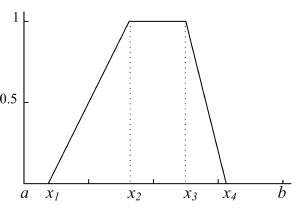
\includegraphics[scale=0.5]{fig/trapese}
		\caption {Trapezoidal MFs}
		\label{fig:trapeze}
	\end{center}
	% Mohammed: Could we remove this figure?
	% Antonio - if we need space, yes, otherwise, it does not matter I think
\end{figure}
And a fuzzy partition with \textit{n} trapezoidal membership functions
is defined by \textit{2n} variables ($x_{1}$,$x_{2}
$,. .., $x_{2n} $ )(Equation \ref{eq:e1}). In this case,
the representation is given by Figure \ref{fig:at}.

\begin{figure}[!ht] 
	\begin{center}
		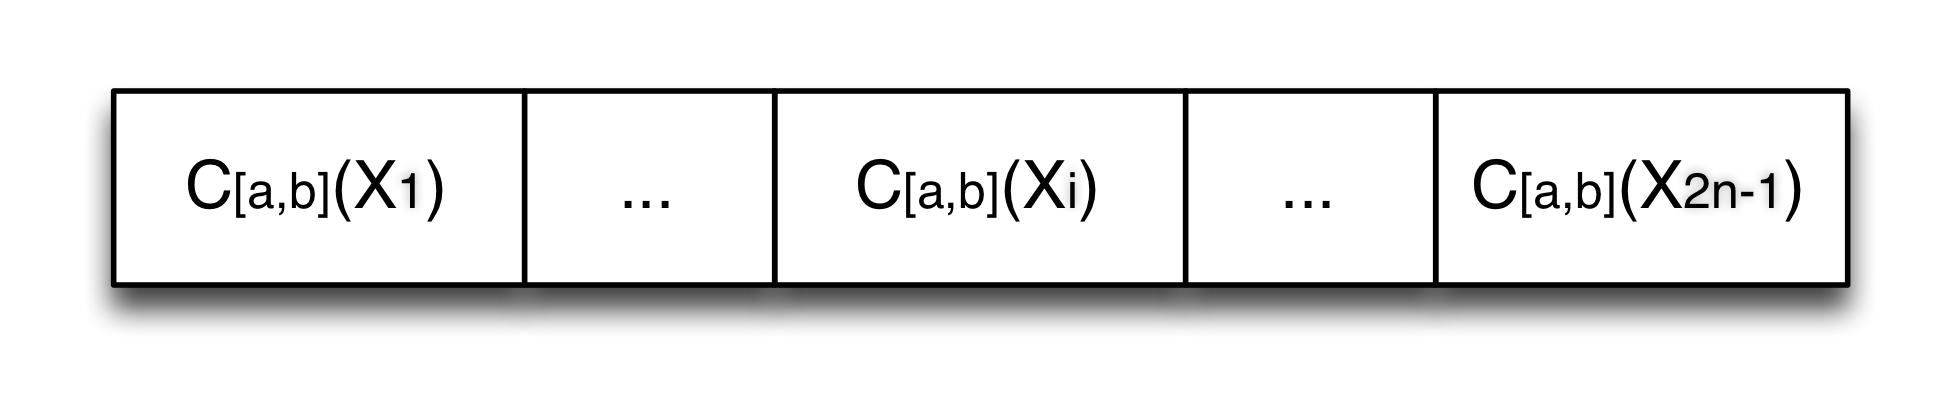
\includegraphics[scale=0.4]{fig/trapezoidal.png}
		\caption {Trapezoidal-shaped MFs coding}
		\label{fig:at}
	\end{center}
\end{figure}
With:
\begin{equation}
	x_{1} \leq x_{2} \leq...\leq x_{2n-1} \leq x_{2n} 	
\end{equation}		
The first variable $x_{1}$ is chosen to be equal to the lower boundary of the range (\textit{a} while $x_{2n}$ is equal to \textit {b}.
\begin{equation} 
	\begin{tabular}{l}
		$\mu_{A1}(x)=  \left \{
		\begin{array}{ll}
		1, &x_{1} \leq x \leq x_{2}\\
		\frac{x_{3} - x}{x_{3} - x_{2}}, &x_{2} \leq x \leq x_{3}\\
		0        , &x > x_{3}\\
		\end{array} 
		\right.$		\\ 	
		$\mu_{Ai}(x)= \left \{
		\begin{array}{ll} 
		0, &x \leq x_{2i-2}\\
		\frac{x - x_{2i-2}}{x_{2i-1} - x_{2i-2}}, &x_{2i-2} \leq x \leq x_{2i-1},n=2,...,i-1\\
		1, & x_{2i-1} \leq x \leq x_{2i}\\
		\frac{x_{2i+1} - x}{x_{2i+1} - x_{2i}},& x_{2i} \leq x \leq x_{2i+1}\\
		0  , &x > x_{2i+1}\\
		\end{array}  
		\right.	$		\\
		$\mu_{An}(x)= \left \{
		\begin{array}{ll} 
		0, &x \leq x_{2n-2}\\
		\frac{x - x_{2n-2}}{x_{2n-1} - x_{2n-2}},& x_{2n-2} \leq x \leq x_{2n-1}\\
		1 ,& x > x_{2n-1} 
		\end{array} 
		\right.$\\
		\label{eq:e1}
	\end{tabular}
\end{equation}

This is the base of the optimization conducted by the Genetic Algorithm, as it is described in the following section.


%%%%%%%%%%%%%%%%%%%%%%%%%%%%  OPTIMISING WITH GAS  %%%%%%%%%%%%%%%%%%%%%%%%%%%%

\section{Genetic Algorithm}
\label{sec:GA_optimization}

We proposed an optimization approach based in Genetic Algorithms (GAs) \cite{GAs_Goldberg89} aiming to find the optimal parameters of the membership functions of the two sub-controllers previously introduced. 

Thus, every individual/chromosome is a vector of 18 values/parameters, 6 per variable, as Figure \ref {fig:cromosome} shows.

\begin{figure*}[!ht]	
	\begin{center}
		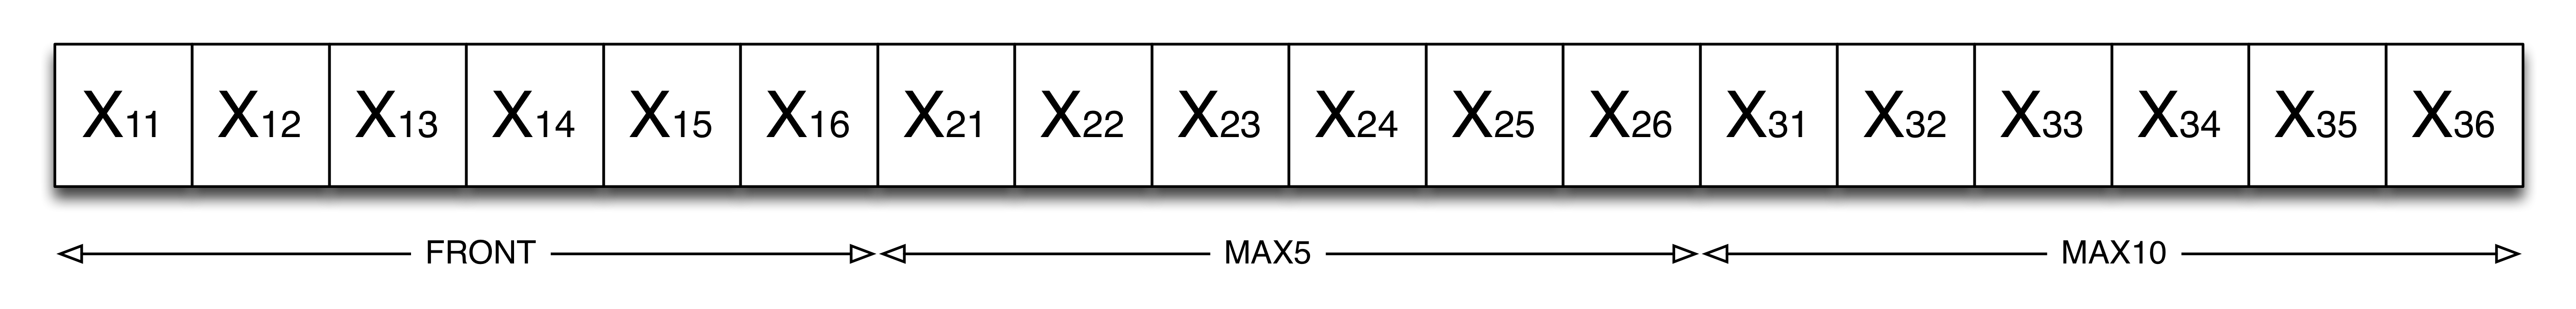
\includegraphics[width=10cm]{fig/chromosome2.png}
		\caption{Chromosome description}
		\label{fig:cromosome}	
	\end{center}	
\end{figure*}

The initialization of the chromosomes (first population) is performed by assigning random values inside a range of variation ($[0,100]$)
\cite{GAs_Goldberg89}, in order to start from feasible values
\cite{salem_evo17}. Since our work requires some precision and the variation interval of each parameter is not well known, we have considered a real coding
implementation \cite{elsayed13} in a vector that includes all variables to optimize.

The overall process is summarized in Figure \ref{fig:ga}. As it can be seen, TORCS is used during the evaluation step of every individual in the evolutionary process.

\begin{figure}[!ht]
	\label{fig:ga}
	\begin{center}
		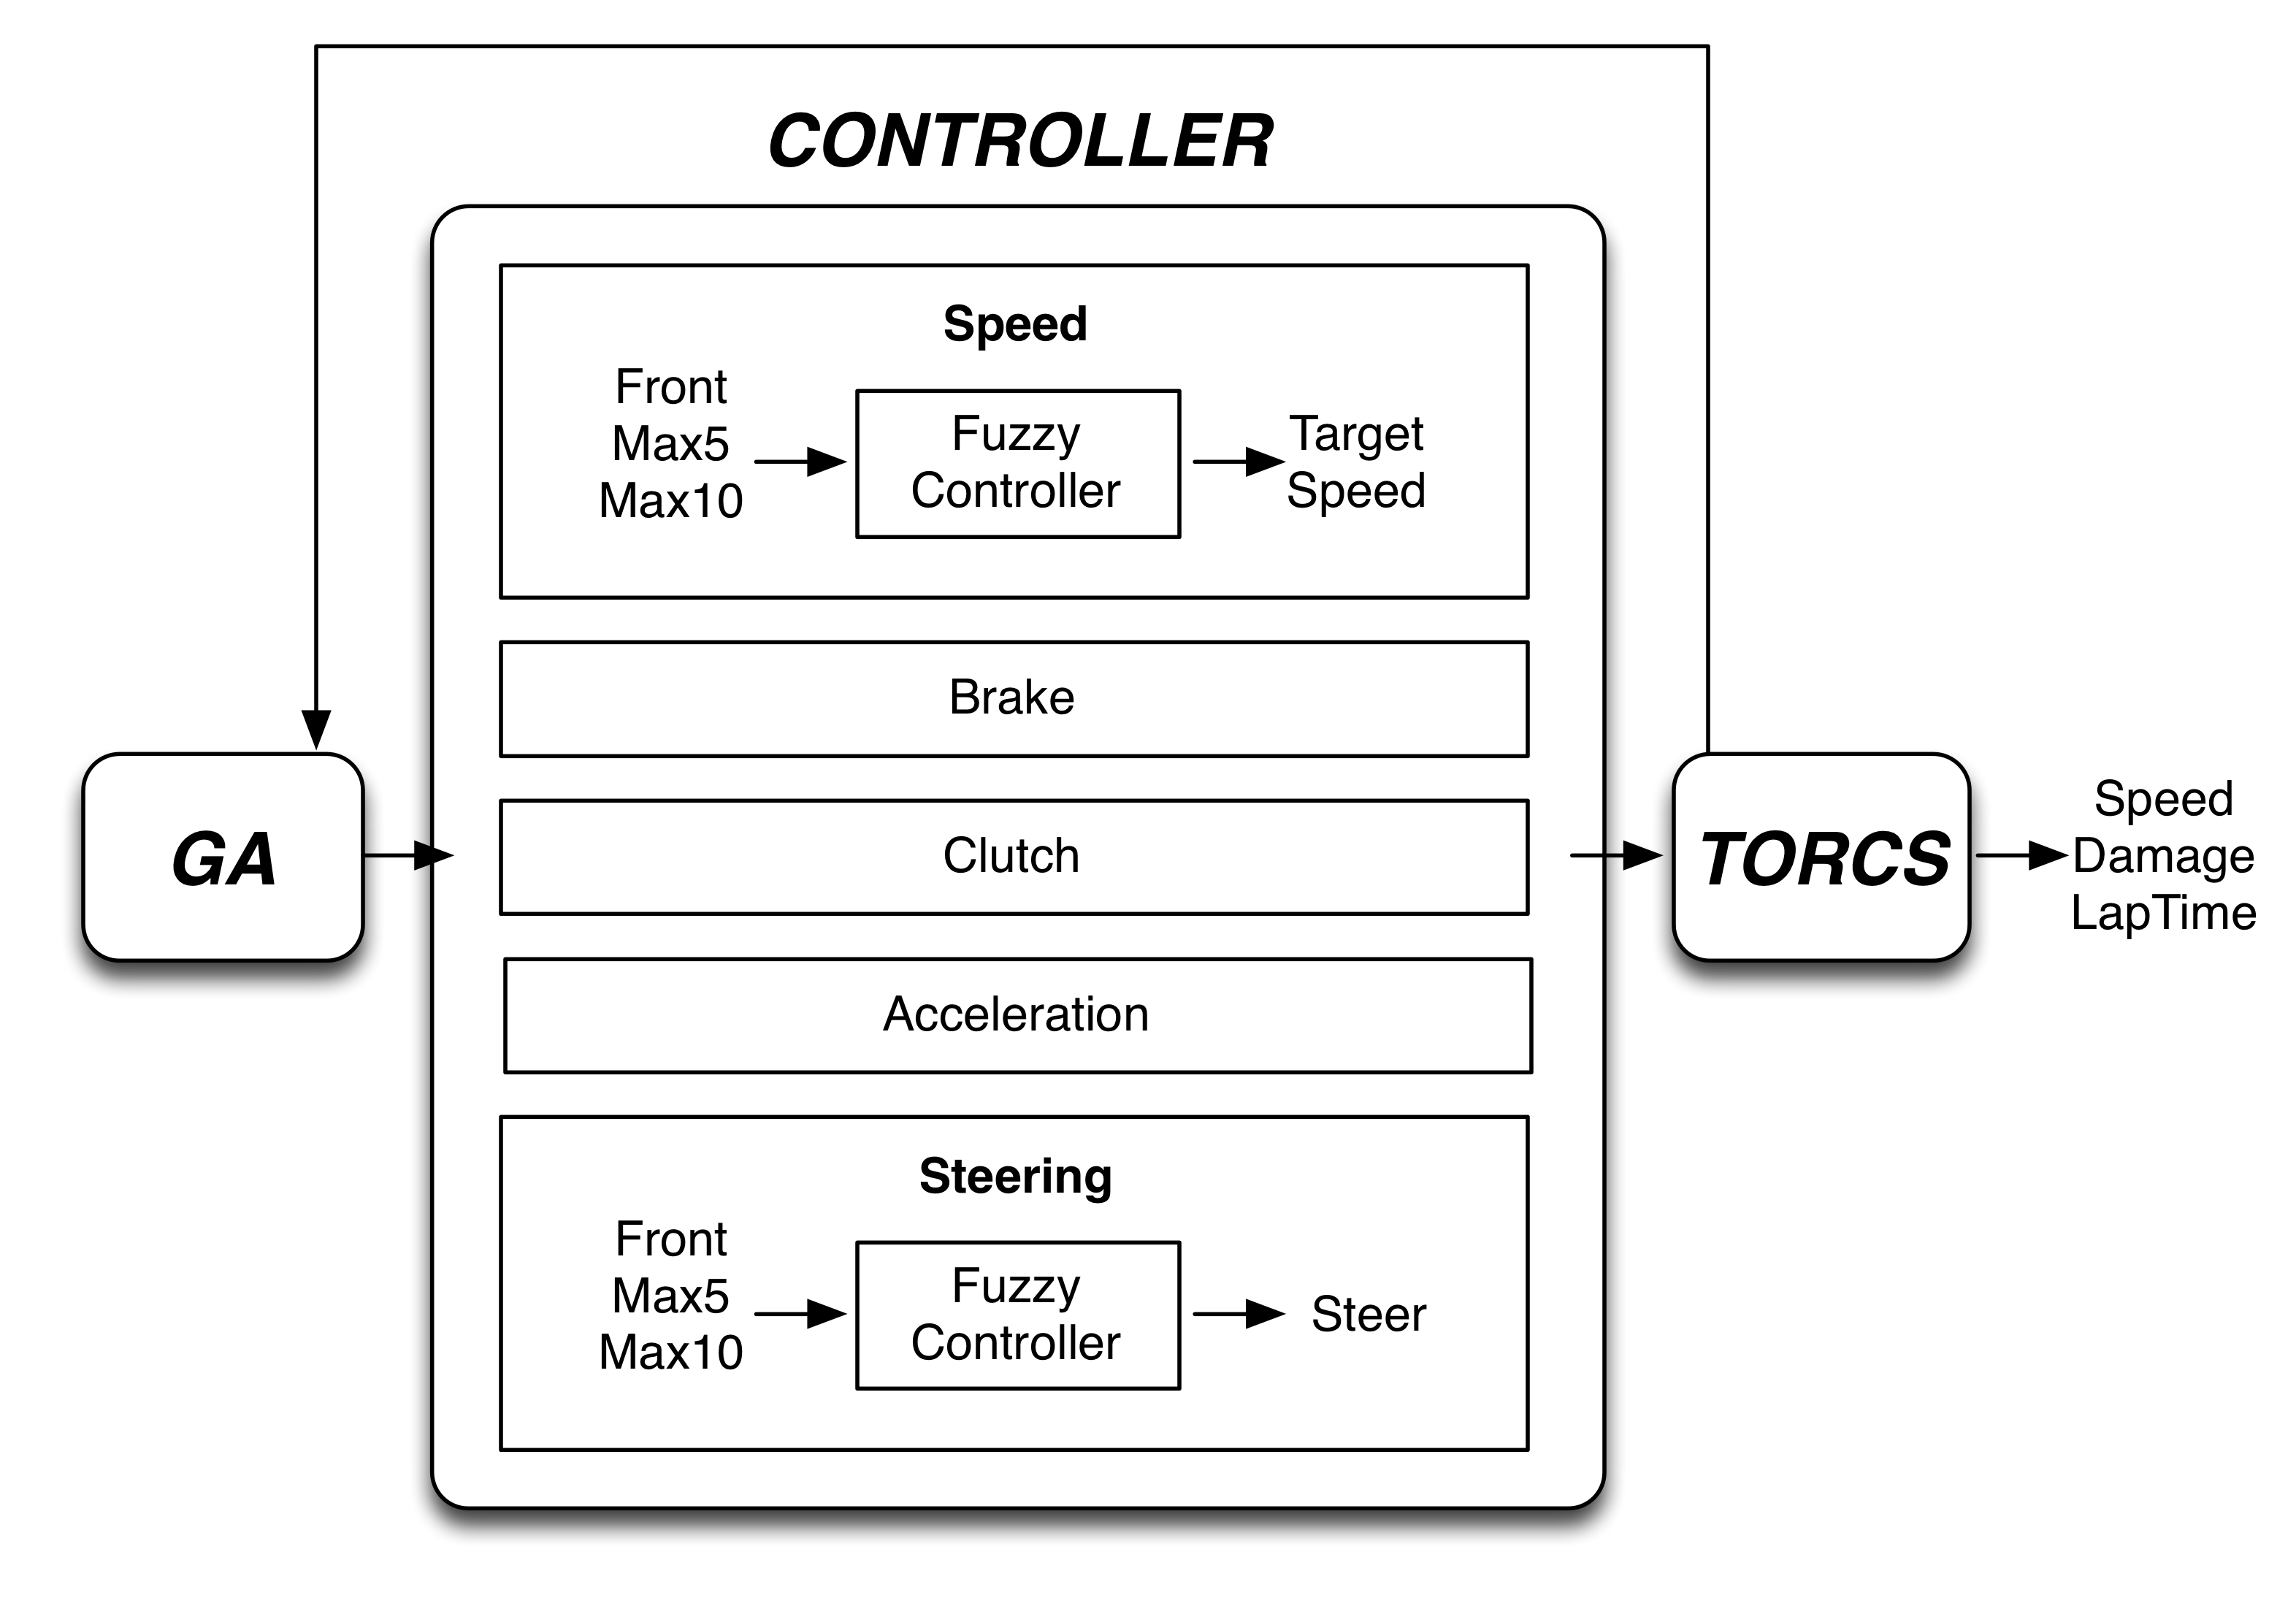
\includegraphics[width=9cm]{fig/flowchart}
	\end{center}
	\caption{Flowchart of  the optimization process of a TORCS fuzzy controller. To evaluate an individual we put the parameter values of the two sub-controllers in the corresponding chromosome, then we launch a race in TORCS with this configuration, obtaining the resulting values of Damage, Top Speed and Mean Lap Time. Individual's fitness value is computed using these values.}
\end{figure}

The evaluation of the individuals is based in different fitness functions, which we have tested in previous works \cite{salem_evo18}. In this study we will consider the one which yielded the best results in our previous paper \cite{salem_cig2018}, namely:

\begin{equation} \label{fit2}
	\begin{array}{lll}
		f_{AVS}= \frac{AVG(Speed)}{Damage+1}
	\end{array}
\end{equation}	

It is a parameter-less approach (no weights in the terms) \cite{Harik-ParameterLess99}, which is also more focused on the real objectives for a driver during a race, rather than the overall target of winning or not,
in order to obtain more `human-like' controllers. It depends on two variables, so the function aims to obtain drivers reaching the highest average speed as possible on the whole track while avoiding damage:

\begin{itemize}
	\item $AVG(Speed)$: pursues a combination of good driving in the difficult zones of the tracks (e.g. curves) and also on easy or straight parts; i.e. considers the overall behavior in the whole track.
	\item $Damage$: aims to create `safe' controllers, as it is mandatory being able to finish the race.
\end{itemize} 

So, the fitness of each candidate solution is computed by injecting its gene values to the parameters of the membership functions of the two fuzzy sub-controllers. The defined autonomous controller is used to drive a
car in a 20 laps race in a circuit without opponents, and the results (Maximum, Minimum and Average speed, Damage) are used to compute the fitness value. 
As the objective of the car controller is to win as many races as
possible, we tried to optimize the most general case by carrying out solo {\em training races}, which will be less sensitive to the presence of noise/uncertainty due to the participation of other controllers \cite{merelo2016statistical}.
The selected track for this evaluation will be one with a combination of curves and straight parts in order to obtain an `all-terrain behaviour'.

With regard to the genetic operators, mutation has remained the same as in previous approaches of our genetic controller, i.e. \textbf{non uniform mutation} \cite{mutation1997}. 

A new \textbf{Pole Position Selection policy} (or race-based selection) has been implemented in this approach, aiming to get better or more reliable individuals/controllers to be parents of the following population. To this end all the individuals are arranged in groups of 10, then some different races of  several laps are simulated using every individual as a controller (with the same car) in a track of TORCS. After every race, the participants obtain different scores depending on their position in the final rank. The best 5 controllers in the sum of all the races are selected as parents for the following offspring.

This way, the best individuals will be selected to reproduce with higher probability. It is not possible to assure they are absolutely the best, due to the uncertainty present in this type of environments, i.e. games against non-deterministic opponents \cite{merelo2016statistical}. However, we argue that this selection policy will be `less sensitive' to that uncertainty (or noise), and thus, it will be fairer and more reliable than an approach purely based on the fitness values. Thus, we think that this proposed selection mechanism would benefit getting a good optimization process.
%Due to the high-demanding time this method is, this race-based selection process is just conducted every 5 generations (not in all of them).


\textbf{BLX-$\alpha$ Crossover operator} \cite{blx2008} has also been added to the GA (instead of previous two-point operator). 
The Blend crossover operator starts by choosing randomly a number from the interval $[x_i-\alpha(y_i-x_i).. y_i+\alpha(y_i-x_i)]$, where $x_i$ and $y_i$ are the
$i^{th}$ parameter values of the parent solutions $x$,$y$ and $x_i < y_i$. See Figure \ref{fig:blxalpha}.

\begin{figure}[!ht]	
	\begin{center}
		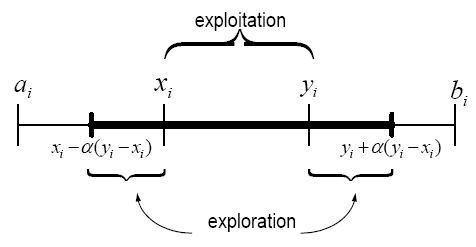
\includegraphics[width=5cm]{fig/blxalpha.jpg}
		\caption{Blend crossover operator ($BLX-\alpha$)}
		\label{fig:blxalpha}	
	\end{center}	
\end{figure}

Thus, this operator is based on the random generation of genes from the associated neighborhood of the genes in the parents. Three generated descendants are different among them and also among them and their parents, leading to a higher exploration factor in the generation of the offspring.
This operator is suitable for real coded genetic algorithms and it has proved to achieve a good balance between exploration and exploitation \cite{blx2008}.

In the Blend crossover operator, the $\alpha$ parameter values can control the exploration/exploitation rate. So, in order to ensure the balance between exploitation and exploration of the search space, $\alpha = 0.5$ could be selected.

In GAs, the search process needs a high exploration rate in the first generations to explore multiple parts of the search space so to obtain high diversity but in the last generations, high exploitation is preferred to ensure the optimal solution.

We have considered two different approaches in the experiments, one taking a  constant value of $\alpha$, and another with a variable scheme, in which the value of $\alpha$ is decreased over the generations (getting sequentially more exploitation and less exploration). Thus, its value is obtained as:

\begin{equation}
	\label{eqalpha}
	\alpha =1-\frac{g}{g_{max}}
\end{equation}

Where $g$ is the current generation and $g_{max}$ is the maximum number pf generations. We think that this approach can achieve an effective balance between exploitation and exploration and therefore, better solutions may be reached.



%%%%%%%%%%%%%%%%%%%%%%%%%%  NEW RIVAL  %%%%%%%%%%%%%%%%%%%%%%%%%%%%

%\section{A New Opponent}  
%\label{sec:new-opponent}

% >>>>>> TODO: Describe "S&PL Controller" -> Antonio  <<<<<<<<<<




%%%%%%%%%%%%%%%%%%%%%%%%%%%%  RESULTS  %%%%%%%%%%%%%%%%%%%%%%%%%%%%

\section{Experiments and results}  
\label{sec:results}

% >>>>>> TODO: Explain the new experiments and results -> Mohammed  <<<<<<<<<<
% TODO: Results with Race-based selection (no BLX-Alpha crossover)
% TODO: Results with Race-Based selection and BLX-Alpha crossover
% TODO: Comparison against the standard controllers in TORCS
% TODO: Comparison against S&PL controller (of all our controllers, if possible)

On the basis of the results of our previous paper \cite{salem_cig2018}, the selection of an appropriate track for training is an important factor in order to obtain competitive bots. \textit{Alpine 2} circuit has been selected for the experiments, since it combines multiple turns with straight parts (See Figure \ref{fig:alpine2_track}).

\begin{figure}[!ht]	
	\begin{center}
		
\includegraphics[width=3cm]{fig/alpine2.jpg}
		\caption{Alpine 2 Track: Slow mountain road. Length: 3773.57m, Width: 10m}
		\label{fig:alpine2_track}	
	\end{center}	
\end{figure}

As in our others studies, we have used the vehicle \textit{car1-tbr1} for our controllers, since it has a moderate performance, which will lead our controller to be prepared to drive in the most usual conditions.

We have evaluated the Genetic Fuzzy Controller (GFC) with the proposed fitness function: $f_{AVS}$ (Equation \ref{fit2}). We have run the algorithm with a population size of 60 individuals. The rest of parameters are: Generations=50, Crossover rate=0.85, Mutation rate=0.09, and 10 different runs per configuration.

New pole position selection has been conducted considering \textit{Alpine 2} track, 5 races and 20 laps per race. 
We have defined a score function based in Formula 1 schema, so the obtained punctuations depend on the car position in the final rank: 1 - 25 points, 2 - 18, 3 - 15, 4 - 12, 5 - 10, 6 - 8, 7 - 6, 8 - 4, 9 - 2, 10 - 1. The the starting grid (initial positions of cars) on these races was set randomly.
Due to the high-demanding time this method is, this race-based selection process has just been performed every 5 generations (not in all of them).

At the end of the evolution (in the last generation) an additional race-based selection process is applied as in previous work \cite{salem_cig2018}. So, the best 10 individuals (according to their fitness) of the final population compete in 5 races (of 5 laps) in the \textit{Alpine 2} track. Formula 1 scores are again applied and the winner will be selected as the best controller of the run.

The evolution process was applied in separate bunches of runs to obtain the following controllers:
\begin{itemize}
	\item $GFC$: Controller  from our previous work \cite{salem_cig2018} 
	% Antonio - the review process is not double-blind. ;)
	using race-based selection only in the final generation and with fitness  $f_{AVS}$ (Equation \ref{fit2}).
	\item $GFC-RS$: A controller obtained by applying the classical two points crossover operator (as in previous works) and race-based selection once every 5 generations and fitness $f_{AVS}$ in the others. 
	\item $GFC-FA$: A controller obtained by applying $BLX-\alpha$ crossover operator with a constant value of $\alpha=0.5$ and race-based selection once every 5 generations and fitness $f_{AVS}$ in the others. 
	\item $GFC-VA$: A controller obtained by applying $BLX-\alpha$ crossover operator with a varying value of $\alpha$ using Equation \ref{eqalpha} and race-based selection once every 5 generations and fitness $f_{AVS}$ in the others. 
\end{itemize}

Once the 10 runs have finished, the obtained 10 best controllers compete again in a similar set of races as those conducted in the last generation of the algorithms, in order to choose the best controller overall per approach, i.e. the best $GFC-RS$, $GFC-FA$ and $GFC-VA$.

% Antonio - Mohammed, are you performing also a race-based selection at the end of the evolution to choose the best of all the controllers, as it was done in GFC?

% If this happens at the end, you should clarify - JJ 
%%%  Mohammed  Yes I do

The final best GFCs (one per approach) are evaluated in some races together in a kind of Formula 1 {\em mini championship}, consisting of 10 races, each one for 20 laps, and with a total of 10 participants per race: the 4 GFCs and also 6 standard bots from TORCS. We have choose two controllers from {\tt tita}, {\tt berniw} and {\tt
	inferno} teams where {\tt berniw} is known by its aggressive overtaking policy while {\tt
	inferno} is the faster one.  The first 5 races are conducted in \textit{Alpine 2} track (used during training/optimization); and the other 5 races took place in \textit{E-Track 5} track (not trained for the new controllers). 
Finally, in order to do it fairer, we have defined an \textit{additional score}, so the controller which gets the fastest lap or the minimum damage in each race is given 5 extra points. The starting grid was again set randomly.

The results of this comparison are shown in Table \ref{tab:chsresults} and summarized graphically in Figure \ref{fig:gfc_races}. 

%
\begin{table*}[ht]
	\centering
	{\scriptsize
		\caption{ Results of the mini-championship with 10 drivers and 10
			races in two different tracks. {\tt tita}, {\tt berniw} and {\tt
				inferno} are example controllers included with the TORCS
			simulator \cite{torcs4}}
		{
			\begin{tabular}{|c||c|c|c|c|c|c||c|c|c|c|c|c||c|}
				\hline
				&\multicolumn{6}{|c|}{Races in \textit{Alpine 2} track (20 laps each)} &	\multicolumn{6}{|c|}{Races in \textit{E-Track 5} track (20 laps each)}&\\
				\cline{2-13}
				Driver&{R1}&{R2}&{R3}&{R4}&{R5}&Track Score&{R6}&{R7}&{R8}& {R9}&{R10}&Track Score& Total Score\\
				\hline
				$GFC$	&	6&	8&	8&	15&15		&52&	12&	15&	10&	10&	15&62&134\\
				$GFC-RS$&	12&	10&	18&	12&12		&64&	10&	8&	12&	25&	8&63&127\\
				$GFC-FA$&	18&	12&	15&	10&10		&65&	15&	12&	25&	15&	25&92&157\\
				$GFC-VA$&	25&	18&	25&	25&18		&111&	25&	18&	15&	18&18	&94&205\\
				$tita1$	&	4&	2&	6&	4&1			&15&	2&	1&	2&	1&	1&7&22\\
				$tita2$	&	2&	1&	2&	2&2			&9&	1&	2&	1&	2&	2&8&17\\
				$inferno1$&	8&	4&	1&	1&6			&20&	4&	4&	6&	8&	6&28&48\\
				$inferno2$&	1&	6&	4&	8&8			&27&	6&	6&	4&	4&	4&24&51\\
				$berniw1$&	10&	25&	10&	18&4		&67&	18&	10&	8&	12&	12&60&127\\
				$berniw2$&	15&	15&	12&	6&25		&73&	8&	25&	18&	6&	10&67&140\\
				\hline
				
			\end{tabular}
		}\label{tab:chsresults}
	}
\end{table*}
%


\begin{figure}[!ht]	
	\begin{center}
		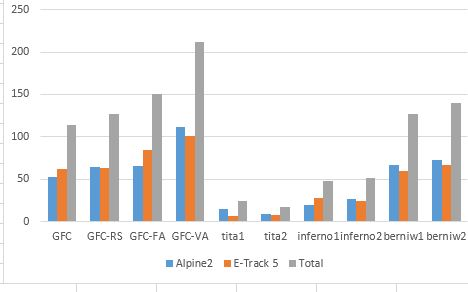
\includegraphics[width=8cm]{fig/gfc_races.jpg}
		\caption{Scores obtained by the different Genetic fuzzy-based controllers in two different tracks.}
		\label{fig:gfc_races}
		% Please don't use screen captures for figures. Also,
		% the little circles around one of the bars make no
		% sense - JJ
	\end{center}
\end{figure}
% Antonio - Mohammed, please, generate the figure without the "dots" in blue bars. Also put the correct name of the track "E-Track 5".
%Mohammed Done
It is clear from the table and figure that the $GFC-VA$ controller
yields the best results in the evaluation process. Indeed, The
proposed controller won three races in Alpine 2 track and has been
ranked in the second place in the two other racing tracks. In the E-Track 5
circuit, it won two races, has been second twice and third in
the last race.

The second controller using the $BLX-\alpha$ (constant value of 0.5)
operator came second in all races. It won one race and was ranked
second in two more and third in three races.
The other races were won by the $berniw$ controller, always a tough rival.
We can notice that the $BLX-\alpha$ based controllers won three out of the five races in the Alpine 2 track used in the selection and were ranked at least in fourth place.
The same results or even  better were obtained for the other track, which is supposed to be unknown for our controllers.

These results confirm the effectiveness and strength of the pole position selection policy used to evaluate individuals as well as to select candidates for crossover. Although this policy has been applied only once every 5 generations due to its time-consuming, it has clearly affected the performance of the obtained controllers looking to the large gap between the results of the $GFC$ controller against $GFC-RS$ one.

This proposed selection policy combined with the $BLX-\alpha$ operator, has boosted the performance of the $GFC-FA$ controller. 
The introduction of a variable $\alpha$ parameter along the
generations in $GFC-VA$ bot has made it possible to better control the
exploration/exploitation ratio during the evolutionary process,
allowing to generate descendants different from their parents in genes
and more efficient than them. 

% -------------------------------------------

%\textbf{Comparison with PSRI controller.}

In order to check the value of our best controller, we have conducted an additional experimentation.

We have considered an opponent from the state of the art, which participated in several Simulated Car Racing Competitions in past editions. 
It was proposed by P{\'e}rez-Li{\'e}bana, S{\'a}ez, Recio and Isasi \cite{EvolvingRuleSystem08} and later refined in the work \cite{PerezEvolvingFuzzy09}. We have baptised it as PSRI in honor of its authors' surnames.

This controller behaves mainly using a Finite State Machine (FSM), defining the main states in which the driver can be (for instance turning, overtaking a rival). The transitions in the FSM are governed by a set of fuzzy rules, based on the information read from different sensors. There is also a classifier module (J48 decision tree), able to analyse the inputs from some sensors in order to predict parts of the track, to anticipate the following actions to perform. The fuzzy rules and also some parameters of the FSM were optimized by means of a NSGA-II algorithm.

As stated, PSRI controller competed in 2009 edition of the Simulated Car Racing Championship \cite{SimulatedCarRacing-2010}, where it was ranked 4th considering the scores obtained in three different Competitions (held at CEC, GECCO and CIG 2009 conferences). It performed on average very well, reaching good scores and positions in several races.

Table \ref{tab:damagespeed} presents a comparison between the two $BLX-\alpha$ genetic based fuzzy controllers presented in this paper, \textbf{$GFC-FA$} and \textbf{$GFC-VA$} with PSRI controller. The results are the average values of $damage$, $MaxSpeed$ and $Speed$ of 10 races in the \textit{Alpine 2} and \textit{E-Track 5} tracks. 

\begin{table}[!ht]
	\centering
	{\scriptsize
		\caption{Average damage and Speed Results of 5 races in
			\textbf{Alpine 2} and 5 races in \textbf{E-Track 5} tracks}
		% Average should always go with standard deviation - JJ
		\label{tab:damagespeed}
		\begin{tabular}{|p{1.65cm}|c|c|c|}
			\hline 
			\multicolumn{4}{|c|}{\textbf{Alpine 2}}  \\	
			\hline  
			& \textbf{$GFC-FA$}&\textbf{$GFC-VA$} & \textbf{$PSRI$}\\					
			\hline \textbf{Average Speed (km/h)}& 187.11&199.65&176.94\\
			\hline \textbf{Max Speed (km/h)}& 225.07&231.91&217.83\\	
			\hline \textbf{Damage}& 126.82& 117.55&131.99 \\	
			\hline \textbf{Won races}&0&4&1\\	
			
			\hline 
		\end{tabular}
		\begin{tabular}{|p{1.65cm}|c|c|c|}
			\hline 
			\multicolumn{4}{|c|}{\textbf{E-Track 5}}  \\
			\hline 
			& \textbf{$GFC-FA$}&\textbf{$GFC-VA$} & \textbf{$PSRI$}\\				
			\hline \textbf{Average Speed (km/h)}& 161.11&170.23&160.89\\
			\hline \textbf{Max Speed  (km/h)}&262.88&270.17&266.54\\	
			\hline \textbf{Damage}&18.12& 14.67&28.09\\	 
			\hline \textbf{Won races}&1&3&1\\	
			\hline 
		\end{tabular}
	}
\end{table} 

The results of the $PSRI$ controller and $GFC-FA$ are very close, they won two and one race respectively among 10. Their average speeds are similar but as for the damage, the controller $GFC-FA$ suffered the minimum because of the inclusion of the variable $damage$ in the fitness evaluation.
The results of the $GFC-VA$ controller are very satisfactory. Indeed, it won 7 races and got the lowest value of damage $117.55$ and $14.67$ for both circuits, the highest average speed $199.65$ and $170.23$.

Looking at these and previous results, we can conclude that the proposed controllers are very successful, due to the new included mechanisms to deal with uncertainty and to perform a more convenient search of the space of solutions.



%%%%%%%%%%%%%%%%%%%%%%%%%%%%  CONCLUSIONS  %%%%%%%%%%%%%%%%%%%%%%%%%%%%
\section{Conclusions and Future Work} 
\label{sec:conclusions}

% >>>>>> TODO: Rewrite this section -> All  <<<<<<<<<<


In this paper we have tried to get winning racing car drivers by
first improving the selection process so that, from time to time,
uncertainty is eliminated by using actual competitions instead of
fitness-based evolution, and second, keep the balance between
exploration and exploitation high, and also variable, by using a fixed
and adaptive version of the BLX-$\alpha$ operator.

The fuzzy genetic controller is subject to uncertainties in the track especially in case of presence of rivals so in order to overcome this problem and thus design a robust and reliable bot, we proposed to apply a \textit{Pole Position Selection policy} where the selection of parents in the evolutionary process is carried out according to the results of a set of mini-championships organized among the individuals of the population, which looks like a car racing tournament selection.
At the same time, and aiming to intensify the exploration process in the search space, we used the $BLX-\alpha$ crossover operator with decreasing values of the $\alpha$ parameter throughout the generations.

The evaluation was performed by comparing the proposed controller with bots of the TORCS platform, yielding very good results.
The other evaluation of our controller was a confrontation with a real bot ($PSRI$ controller), which participated in several Simulated Car Racing Competitions. In this case, the BLX operator and the new selection policy have had a lot of impact in helping our controller to win three quarters of the races by getting the lowest damage, average speed and maximum speed values.

These results let us to think that our controller could have reached a very good rank in the Simulated Car Racing Competition, which is unfortunately over since 2013. Anyway, we think that the findings of this study (and previous ones) could be applied successfully to other car racing simulators, such as those used in current eSports Competitions, such as iRace (https://www.iracing.com/).

As future lines of work, this controller can be improved in some ways:
We can extend the selection policy to all generations while overcoming the computation time drawback by means of a parallel implementation.
We can also explore other parameter-less fitness functions to evaluate individuals including other factors affecting the performance of the car.
Another perspective is to use multiple tracks (instead of just one) in the selection process in order to train a more general controller, able to deal with many different situations.

\section*{Acknowledgments}

This work has been supported in part by: Ministerio espa\~{n}ol de
Econom\'{\i}a y Competitividad under projects  TIN2017-85727-C4-2-P (UGR-DeepBio) and TEC2015-68752 (also funded by FEDER).

\bibliographystyle{IEEEtranS}
\bibliography{fuzzy_torcs,geneura}


% Computer Society journal (but not conference!) papers do something unusual
% with the very first section heading (almost always called "Introduction").
% They place it ABOVE the main text! IEEEtran.cls does not automatically do
% this for you, but you can achieve this effect with the provided
% \IEEEraisesectionheading{} command. Note the need to keep any \label that
% is to refer to the section immediately after \section in the above as
% \IEEEraisesectionheading puts \section within a raised box.




% The very first letter is a 2 line initial drop letter followed
% by the rest of the first word in caps (small caps for compsoc).
% 
% form to use if the first word consists of a single letter:
% \IEEEPARstart{A}{demo} file is ....
% 
% form to use if you need the single drop letter followed by
% normal text (unknown if ever used by the IEEE):
% \IEEEPARstart{A}{}demo file is ....
% 
% Some journals put the first two words in caps:
% \IEEEPARstart{T}{his demo} file is ....
% 
% Here we have the typical use of a "T" for an initial drop letter
% and "HIS" in caps to complete the first word.
%\IEEEPARstart{T}{his} demo file is intended to serve as a ``starter file''
%for IEEE Computer Society journal papers produced under \LaTeX\ using
%IEEEtran.cls version 1.8b and later.
% You must have at least 2 lines in the paragraph with the drop letter
% (should never be an issue)
%I wish you the best of success.
%
%\hfill mds
% 
%\hfill August 26, 2015
%
%\subsection{Subsection Heading Here}
%Subsection text here.

% needed in second column of first page if using \IEEEpubid
%\IEEEpubidadjcol

%\subsubsection{Subsubsection Heading Here}
%Subsubsection text here.


% An example of a floating figure using the graphicx package.
% Note that \label must occur AFTER (or within) \caption.
% For figures, \caption should occur after the \includegraphics.
% Note that IEEEtran v1.7 and later has special internal code that
% is designed to preserve the operation of \label within \caption
% even when the captionsoff option is in effect. However, because
% of issues like this, it may be the safest practice to put all your
% \label just after \caption rather than within \caption{}.
%
% Reminder: the "draftcls" or "draftclsnofoot", not "draft", class
% option should be used if it is desired that the figures are to be
% displayed while in draft mode.
%
%\begin{figure}[!t]
%\centering
%\includegraphics[width=2.5in]{myfigure}
% where an .eps filename suffix will be assumed under latex, 
% and a .pdf suffix will be assumed for pdflatex; or what has been declared
% via \DeclareGraphicsExtensions.
%\caption{Simulation results for the network.}
%\label{fig_sim}
%\end{figure}

% Note that the IEEE typically puts floats only at the top, even when this
% results in a large percentage of a column being occupied by floats.
% However, the Computer Society has been known to put floats at the bottom.


% An example of a double column floating figure using two subfigures.
% (The subfig.sty package must be loaded for this to work.)
% The subfigure \label commands are set within each subfloat command,
% and the \label for the overall figure must come after \caption.
% \hfil is used as a separator to get equal spacing.
% Watch out that the combined width of all the subfigures on a 
% line do not exceed the text width or a line break will occur.
%
%\begin{figure*}[!t]
%\centering
%\subfloat[Case I]{\includegraphics[width=2.5in]{box}%
%\label{fig_first_case}}
%\hfil
%\subfloat[Case II]{\includegraphics[width=2.5in]{box}%
%\label{fig_second_case}}
%\caption{Simulation results for the network.}
%\label{fig_sim}
%\end{figure*}
%
% Note that often IEEE papers with subfigures do not employ subfigure
% captions (using the optional argument to \subfloat[]), but instead will
% reference/describe all of them (a), (b), etc., within the main caption.
% Be aware that for subfig.sty to generate the (a), (b), etc., subfigure
% labels, the optional argument to \subfloat must be present. If a
% subcaption is not desired, just leave its contents blank,
% e.g., \subfloat[].


% An example of a floating table. Note that, for IEEE style tables, the
% \caption command should come BEFORE the table and, given that table
% captions serve much like titles, are usually capitalized except for words
% such as a, an, and, as, at, but, by, for, in, nor, of, on, or, the, to
% and up, which are usually not capitalized unless they are the first or
% last word of the caption. Table text will default to \footnotesize as
% the IEEE normally uses this smaller font for tables.
% The \label must come after \caption as always.
%
%\begin{table}[!t]
%% increase table row spacing, adjust to taste
%\renewcommand{\arraystretch}{1.3}
% if using array.sty, it might be a good idea to tweak the value of
% \extrarowheight as needed to properly center the text within the cells
%\caption{An Example of a Table}
%\label{table_example}
%\centering
%% Some packages, such as MDW tools, offer better commands for making tables
%% than the plain LaTeX2e tabular which is used here.
%\begin{tabular}{|c||c|}
%\hline
%One & Two\\
%\hline
%Three & Four\\
%\hline
%\end{tabular}
%\end{table}


% Note that the IEEE does not put floats in the very first column
% - or typically anywhere on the first page for that matter. Also,
% in-text middle ("here") positioning is typically not used, but it
% is allowed and encouraged for Computer Society conferences (but
% not Computer Society journals). Most IEEE journals/conferences use
% top floats exclusively. 
% Note that, LaTeX2e, unlike IEEE journals/conferences, places
% footnotes above bottom floats. This can be corrected via the
% \fnbelowfloat command of the stfloats package.




%\section{Conclusion}
%The conclusion goes here.





% if have a single appendix:
%\appendix[Proof of the Zonklar Equations]
% or
%\appendix  % for no appendix heading
% do not use \section anymore after \appendix, only \section*
% is possibly needed

% use appendices with more than one appendix
% then use \section to start each appendix
% you must declare a \section before using any
% \subsection or using \label (\appendices by itself
% starts a section numbered zero.)
%


%\appendices
%\section{Proof of the First Zonklar Equation}
%Appendix one text goes here.

% you can choose not to have a title for an appendix
% if you want by leaving the argument blank
%\section{}
%Appendix two text goes here.


% use section* for acknowledgment
%\ifCLASSOPTIONcompsoc
%  % The Computer Society usually uses the plural form
%  \section*{Acknowledgments}
%\else
%  % regular IEEE prefers the singular form
%  \section*{Acknowledgment}
%\fi


%The authors would like to thank...


% Can use something like this to put references on a page
% by themselves when using endfloat and the captionsoff option.
%\ifCLASSOPTIONcaptionsoff
%  \newpage
%\fi



% trigger a \newpage just before the given reference
% number - used to balance the columns on the last page
% adjust value as needed - may need to be readjusted if
% the document is modified later
%\IEEEtriggeratref{8}
% The "triggered" command can be changed if desired:
%\IEEEtriggercmd{\enlargethispage{-5in}}

% references section

% can use a bibliography generated by BibTeX as a .bbl file
% BibTeX documentation can be easily obtained at:
% http://mirror.ctan.org/biblio/bibtex/contrib/doc/
% The IEEEtran BibTeX style support page is at:
% http://www.michaelshell.org/tex/ieeetran/bibtex/
%\bibliographystyle{IEEEtran}
% argument is your BibTeX string definitions and bibliography database(s)
%\bibliography{IEEEabrv,../bib/paper}
%
% <OR> manually copy in the resultant .bbl file
% set second argument of \begin to the number of references
% (used to reserve space for the reference number labels box)
%\begin{thebibliography}{1}
%
%\bibitem{IEEEhowto:kopka}
%H.~Kopka and P.~W. Daly, \emph{A Guide to \LaTeX}, 3rd~ed.\hskip 1em plus
%  0.5em minus 0.4em\relax Harlow, England: Addison-Wesley, 1999.
%
%\end{thebibliography}

% biography section
% 
% If you have an EPS/PDF photo (graphicx package needed) extra braces are
% needed around the contents of the optional argument to biography to prevent
% the LaTeX parser from getting confused when it sees the complicated
% \includegraphics command within an optional argument. (You could create
% your own custom macro containing the \includegraphics command to make things
% simpler here.)
%\begin{IEEEbiography}[{\includegraphics[width=1in,height=1.25in,clip,keepaspectratio]{mshell}}]{Michael Shell}
% or if you just want to reserve a space for a photo:

\begin{IEEEbiography}{Mohammed Salem}
Biography text here.
\end{IEEEbiography}

% if you will not have a photo at all:
\begin{IEEEbiographynophoto}{Antonio~M.~Mora}
Biography text here.
\end{IEEEbiographynophoto}

% insert where needed to balance the two columns on the last page with
% biographies
%\newpage





\begin{IEEEbiographynophoto}{Juan~J.~Merelo}
Biography text here.
\end{IEEEbiographynophoto}

% You can push biographies down or up by placing
% a \vfill before or after them. The appropriate
% use of \vfill depends on what kind of text is
% on the last page and whether or not the columns
% are being equalized.

%\vfill

% Can be used to pull up biographies so that the bottom of the last one
% is flush with the other column.
%\enlargethispage{-5in}



% that's all folks
\end{document}


